\textbf{Целью} данной работы является ознакомление с существующими методиками предварительной оценки параметров программного проекта и практическая оценка затрат на примере методики COCOMO.

\section*{Модель оценки стоимости СОСОМО}

Одной из моделей оценки таких параметров проекта, как трудозатраты, длительность и стоимость, является конструктивная модель оценки стоимости COCOMO. При вычислении характеристик проекта по данной модели используются множители и показатели степени, полученные на основе анализа данных большого количества практически реализованных проектов.

Трудозатраты проекта --- число человеко-месяцев --- определяются по следующей формуле:

\begin{equation}
	\text{Трудозатраты } = C1 \cdot EAF \cdot (\text{Размер})^{P1}, \text{ где}
\end{equation}

\begin{itemize}
	\item $C1$ --- масштабирующий коэффициент;
	\item $EAF$ --- уточняющий фактор, характеризующий предметную область, персонал, среду и инструментарий, используемый для создания рабочих продуктов процесса, который является результатом учета 15 драйверов затрат;
	\item Размер --- число исходных инструкций конечного продукта, измеряемое в тысячах строк кода $KLOC$;
	\item $P1$ --- показатель степени, характеризующий экономию при больших масштабах, присущую тому процессу, который используется для создания конечного продукта; в частности, способность процесса избегать непроизводительных видов деятельности (доработок, бюрократических проволочек, накладных расходов на взаимодействие).
\end{itemize}

Время проекта --- общее количество месяцев --- определяется по следующей формуле:

\begin{equation}
	\text{Время } = C2 \cdot(\text{Трудозатраты})^{P2}, \text{ где}
\end{equation}

\begin{itemize}
	\item $C2$ --- масштабирующий коэффициент для сроков исполнения;
	\item $P2$ --- показатель степени, который характеризует инерцию и распараллеливание, присущие управлению разработкой программного обеспечения.
\end{itemize}

При этом могут поддерживаться разные режимы проекта, драйверы затрат выбираются в соответствии с характеристиками разрабатываемого проекта.

Для выполнения заданий 1 и 2, представленных далее, было разработано программное приложение для расчета параметров проекта по методике COCOMO.

\section*{Задание 1}

\subsubsection*{Условие}

Исследовать степень влияния различных драйверов затрат на трудоемкость (РМ) и время разработки (ТМ) для модели COCOMO. Для этого проанализировать, как меняется трудоемкость и время выполнения проекта при различных уровнях автоматизации среды:

\begin{itemize}
	\item драйвер MODP --- использование современных методов;
	\item драйвер TOOL --- использование программных инструментов;
\end{itemize}

\noindentи разном уровне способностей ключевых членов команды:

\begin{itemize}
	\item драйвер ACAP --- способности аналитика;
	\item драйвер PCAP --- способности программиста.
\end{itemize}

Взять за основу любой из типов проекта (обычный, встроенный или промежуточный) и при фиксированном значении размера программного кода (SIZE) получить значения PM и ТМ, изменяя значения указанных драйверов от очень низких до очень высоких. Результаты исследований оформить графически и сделать соответствующие выводы. 

При необходимости сократить срок выполнения проекта, что повлияет больше: способности персонала или параметры среды? 

При высоком уровне автоматизации (оба драйвера MODP и TOOL высокие) что окажет большее влияние на трудоемкость и время выполнения: высокая сложность продукта (параметр CPLX) или высокие ограничения на требуемые сроки разработки (параметр SCED)?

\subsubsection*{Выполнение}

На рисунке \ref{img:task11} показаны графики зависимости трудозатрат и времени выполнения от атрибутов проекта MODP и TOOL и атрибутов персонала ACAP и PCAP при промежуточном режиме проекта.

На рисунке \ref{img:task12} показаны графики зависимости трудозатрат и времени выполнения от атрибута программного продукта CPLX и атрибута проекта SCED при высоких значениях драйверов MODP и TOOL и промежуточном режиме проекта.

\begin{figure}[H]
	\begin{center}
		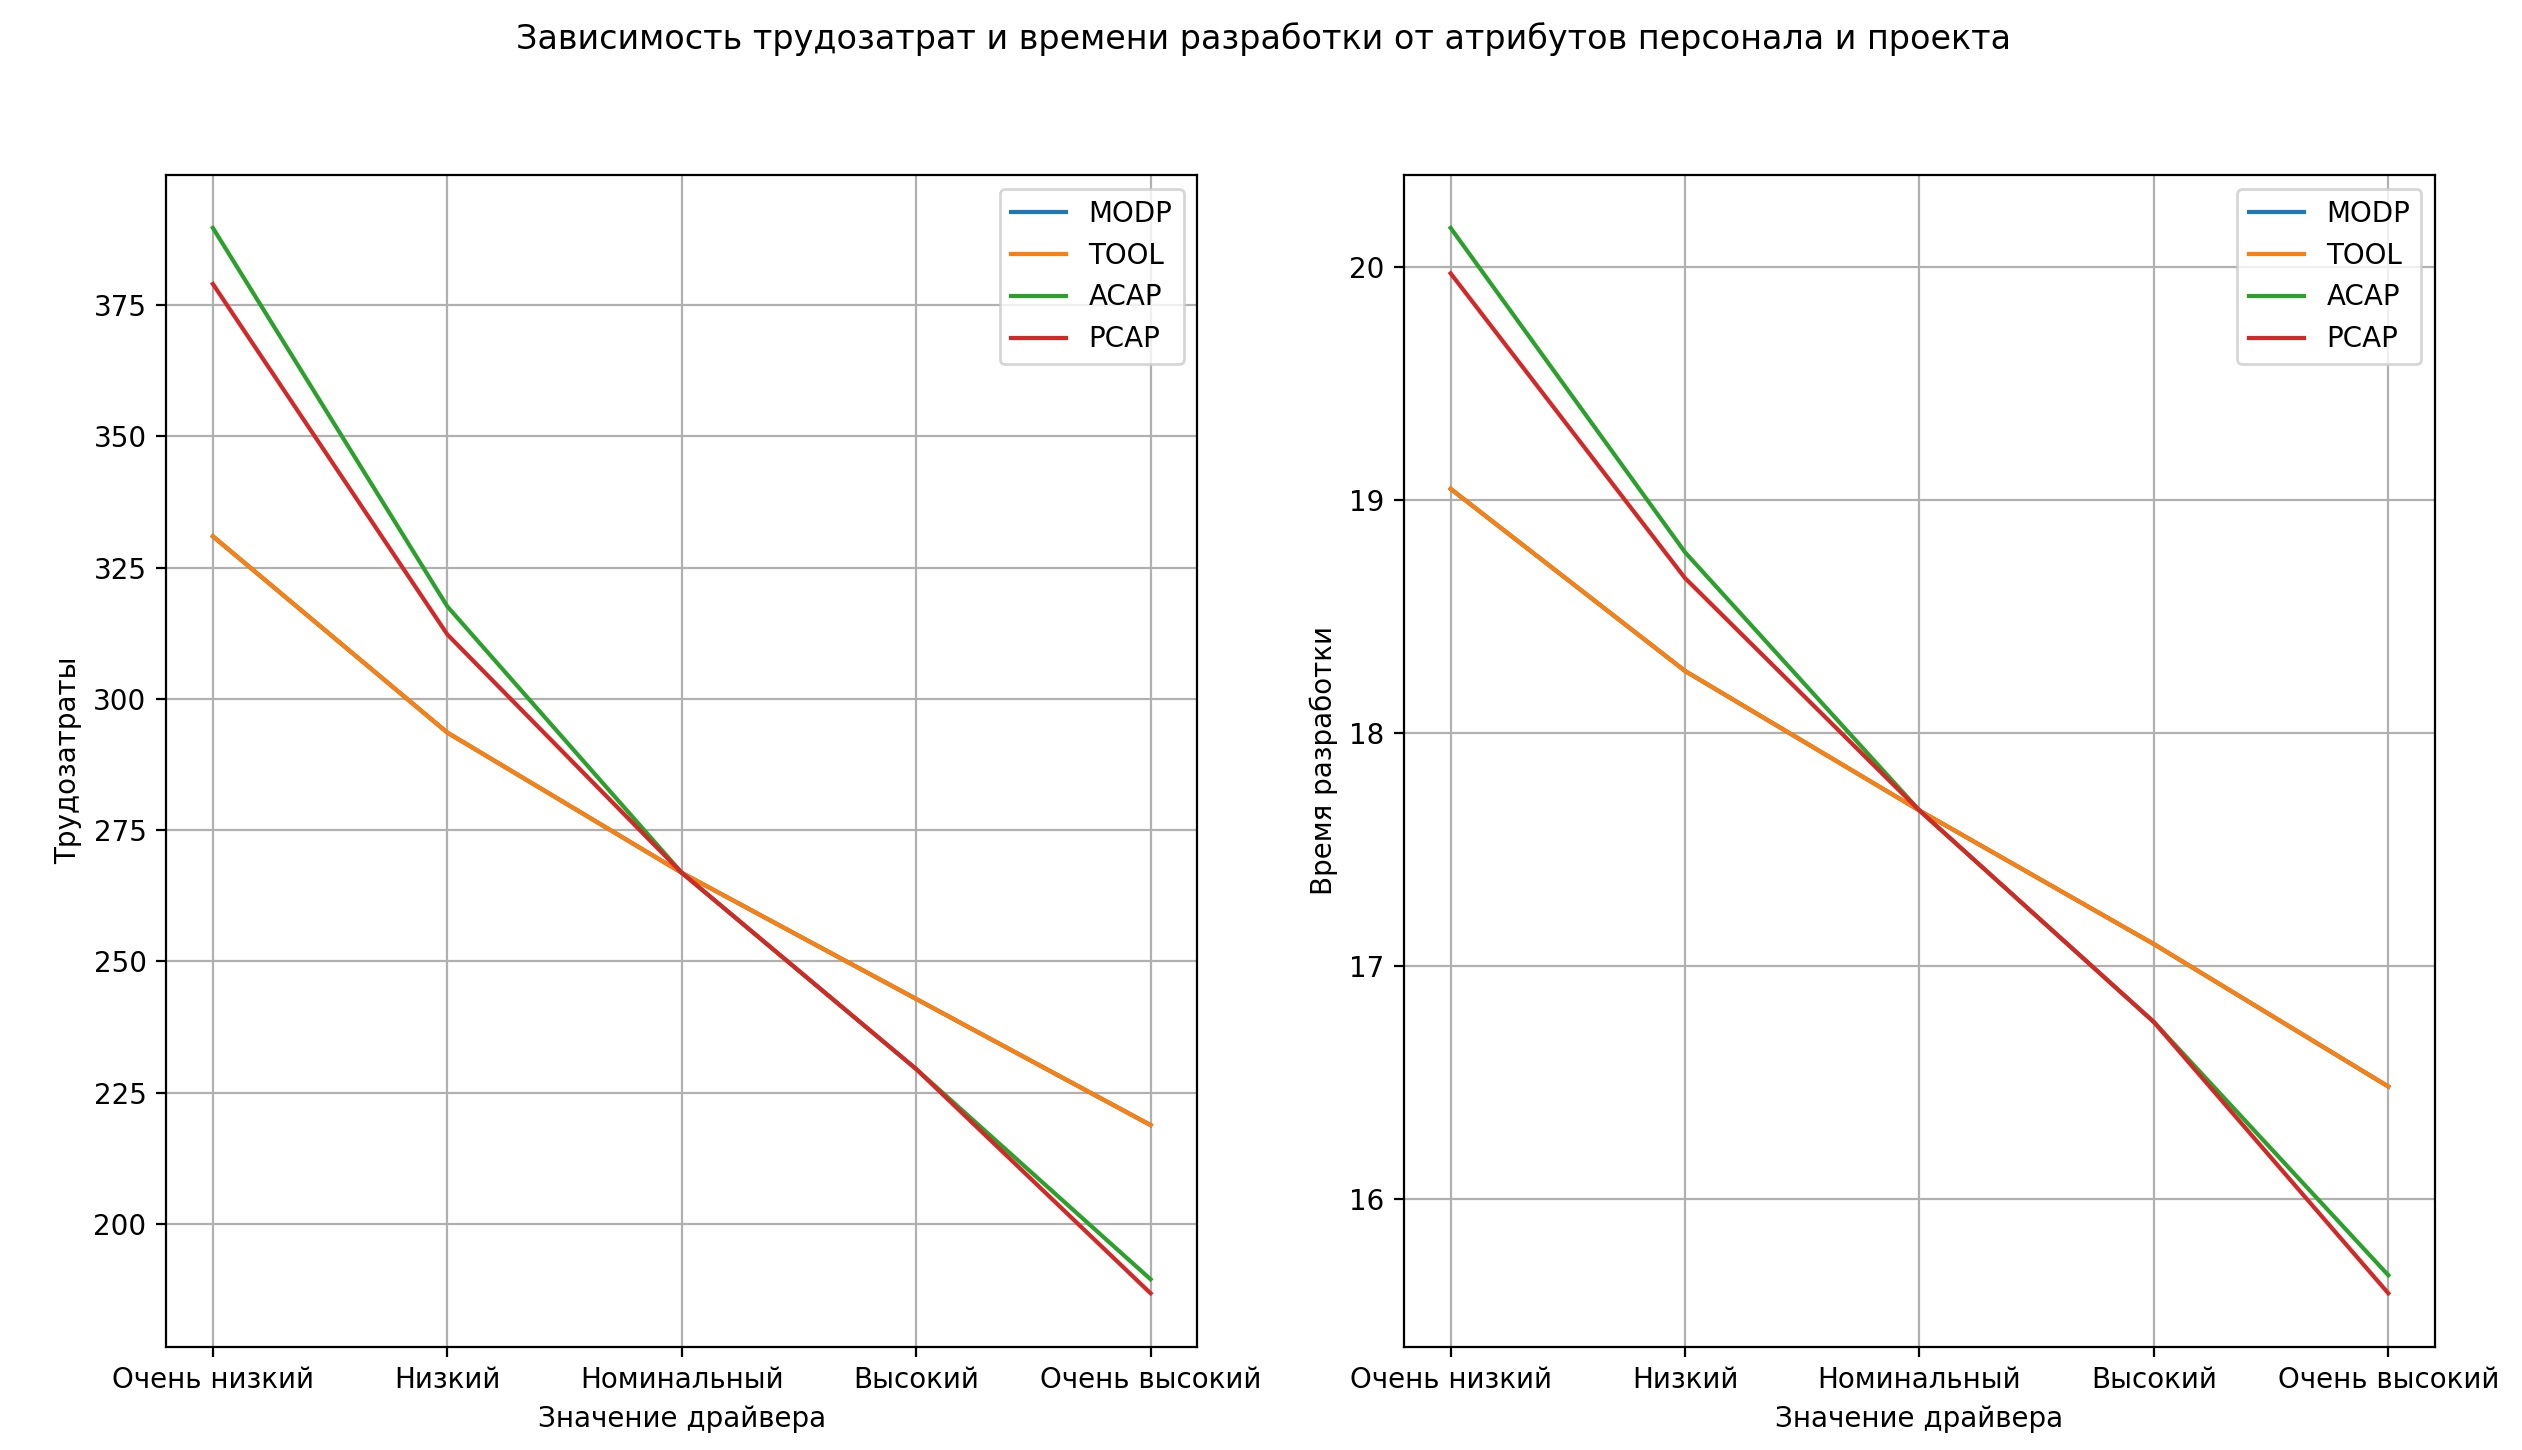
\includegraphics[scale=0.19]{inc/img/task11.jpg}
	\end{center}
	\captionsetup{justification=centering}
	\caption{Исследование влияния атрибутов персонала и проекта на трудоемкость и время выполнения}
	\label{img:task11}
\end{figure}

\subsubsection*{Выводы}

Анализ графиков показал:

\begin{itemize}
	\item с увеличением значений использования современных методов MODP, использования программных инструментов TOOL, способностей аналитика ACAP и способностей программиста PCAP трудоемкость и время разработки уменьшаются, при этом:
		\begin{itemize}
			\item атрибуты персонала больше влияют на трудоемкость и время разработки, чем атрибуты проекта;
			\item влияние способностей аналитика ACAP больше влияния способностей программиста PCAP;
			\item влияние использования современных методов MODP совпадает с влиянием использования программных инструментов TOOL;
		\end{itemize}
	\item исходя из предыдущих выводов: при необходимости сократить срок выполнения проекта больше повлияют способности персонала;
	\item с увеличением значений сложности продукта CPLX трудоемкость и время разработки увеличиваются;
	\item при высоком уровне автоматизации на трудоемкость и время выполнения высокая сложность оказывает большее влияние, чем высокие ограничения на требуемые сроки разработки.
\end{itemize}

\begin{figure}[H]
	\begin{center}
		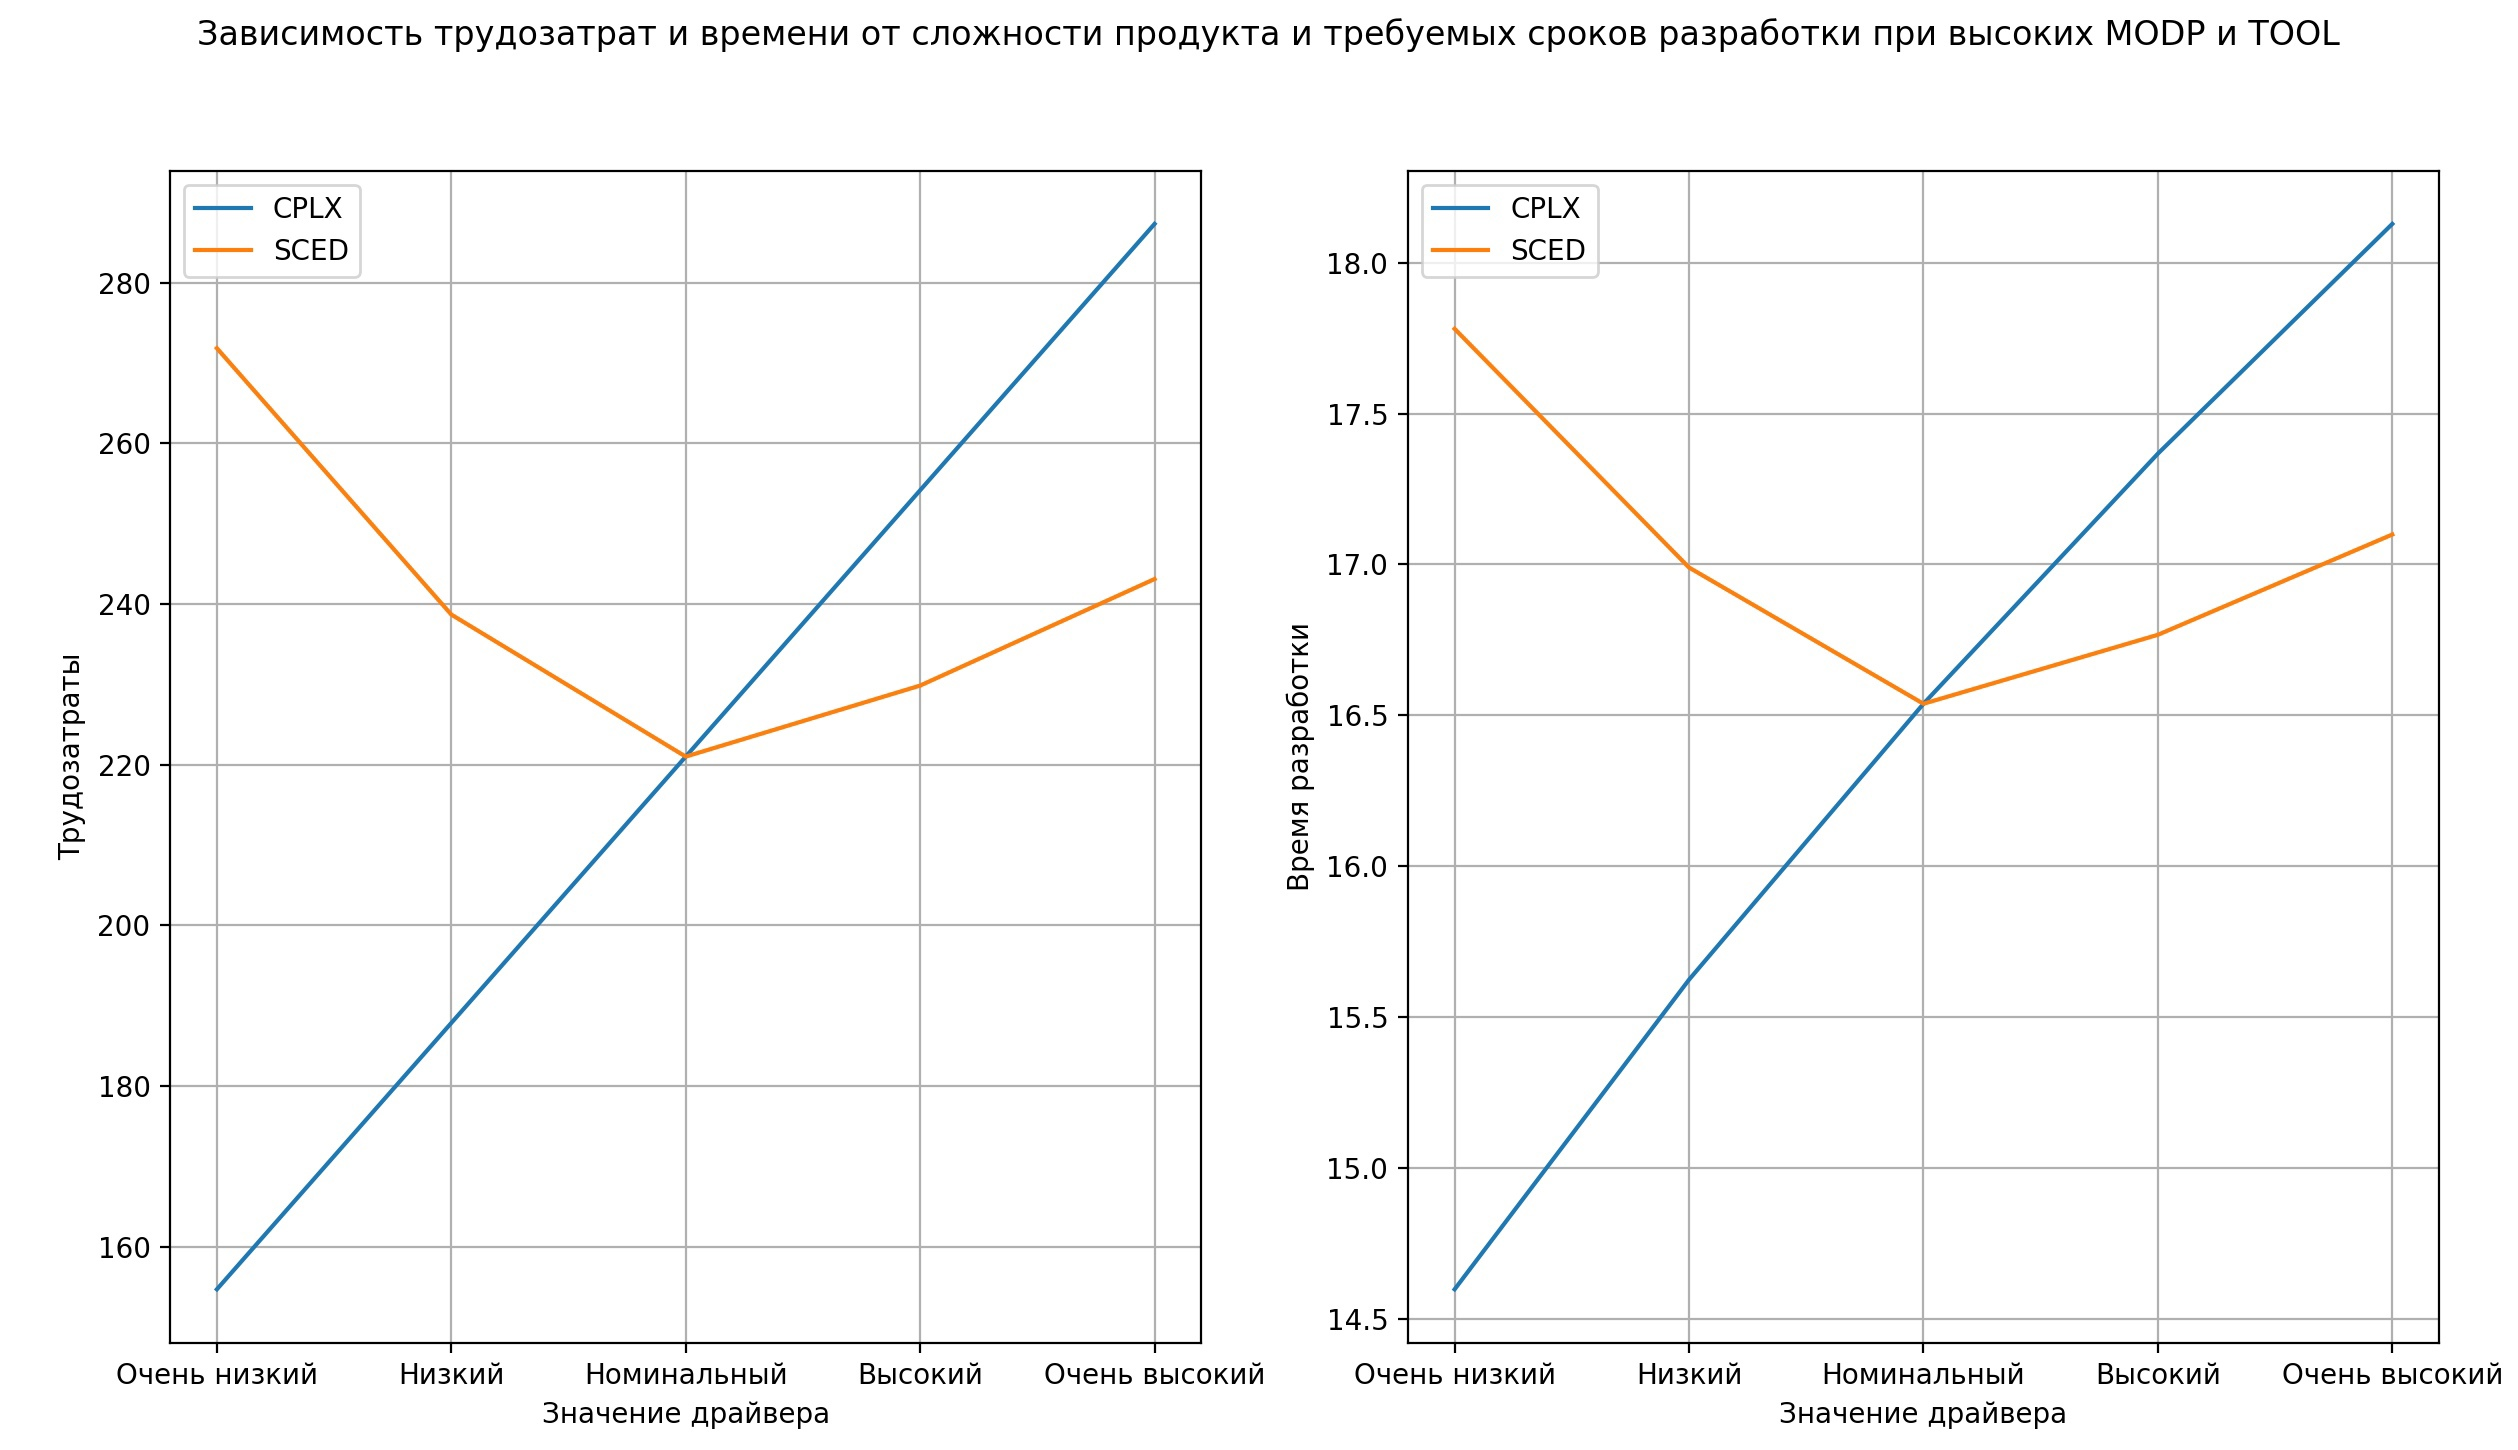
\includegraphics[scale=0.19]{inc/img/task12.jpg}
	\end{center}
	\captionsetup{justification=centering}
	\caption{Исследование влияния сложности продукта и требуемых сроков разработки при высоком уровне автоматизации}
	\label{img:task12}
\end{figure}

\section*{Задание 2}

\subsubsection*{Условие}

При разработке программного проекта его размер оценивается примерно в 55 KLOC. Этот проект будет представлять собой Web-систему, снабженную устойчивой серверной базой данных. Предполагается применение промежуточного варианта. Проект предполагает создание продукта средней сложности с номинальными требованиями по надежности, но с расширенной базой данных. Квалификация персонала средняя. Однако способности аналитика высокие. Оценить параметры проекта.

\subsubsection*{Выполнение}

Из условия:

\begin{itemize}
	\item режим проекта --- промежуточный;
	\item $KLOC = 55$;
	\item размер базы данных DATA --- высокий;
	\item способности аналитика ACAP --- высокие;
	\item прочие драйверы затрат --- номинальные.
\end{itemize}

Тогда:

\begin{itemize}
	\item $C1 = 3, P1 = 1.12$;
	\item $EAF = 1^{13} \cdot 1.08 \cdot 0.86 = 0.9288$;
	\item $\text{Трудозатраты } = 3 \cdot 0.9288 \cdot 55^{1.12} = 247.88 \text{ человеко-месяца}$ (без планирования и определения требований);
	\item $C2 = 2.5, P2 = 0.35$;
	\item $\text{Время } = 2.5 \cdot 247.88^{0.35} = 17.22 \text{ месяцев}$  (без планирования и определения требований).
\end{itemize}

На рисунке \ref{img:task2} приведены распределение работ и времени по стадиям жизненного цикла и распределение работ по видам деятельности WBS.

\begin{figure}[H]
	\begin{center}
		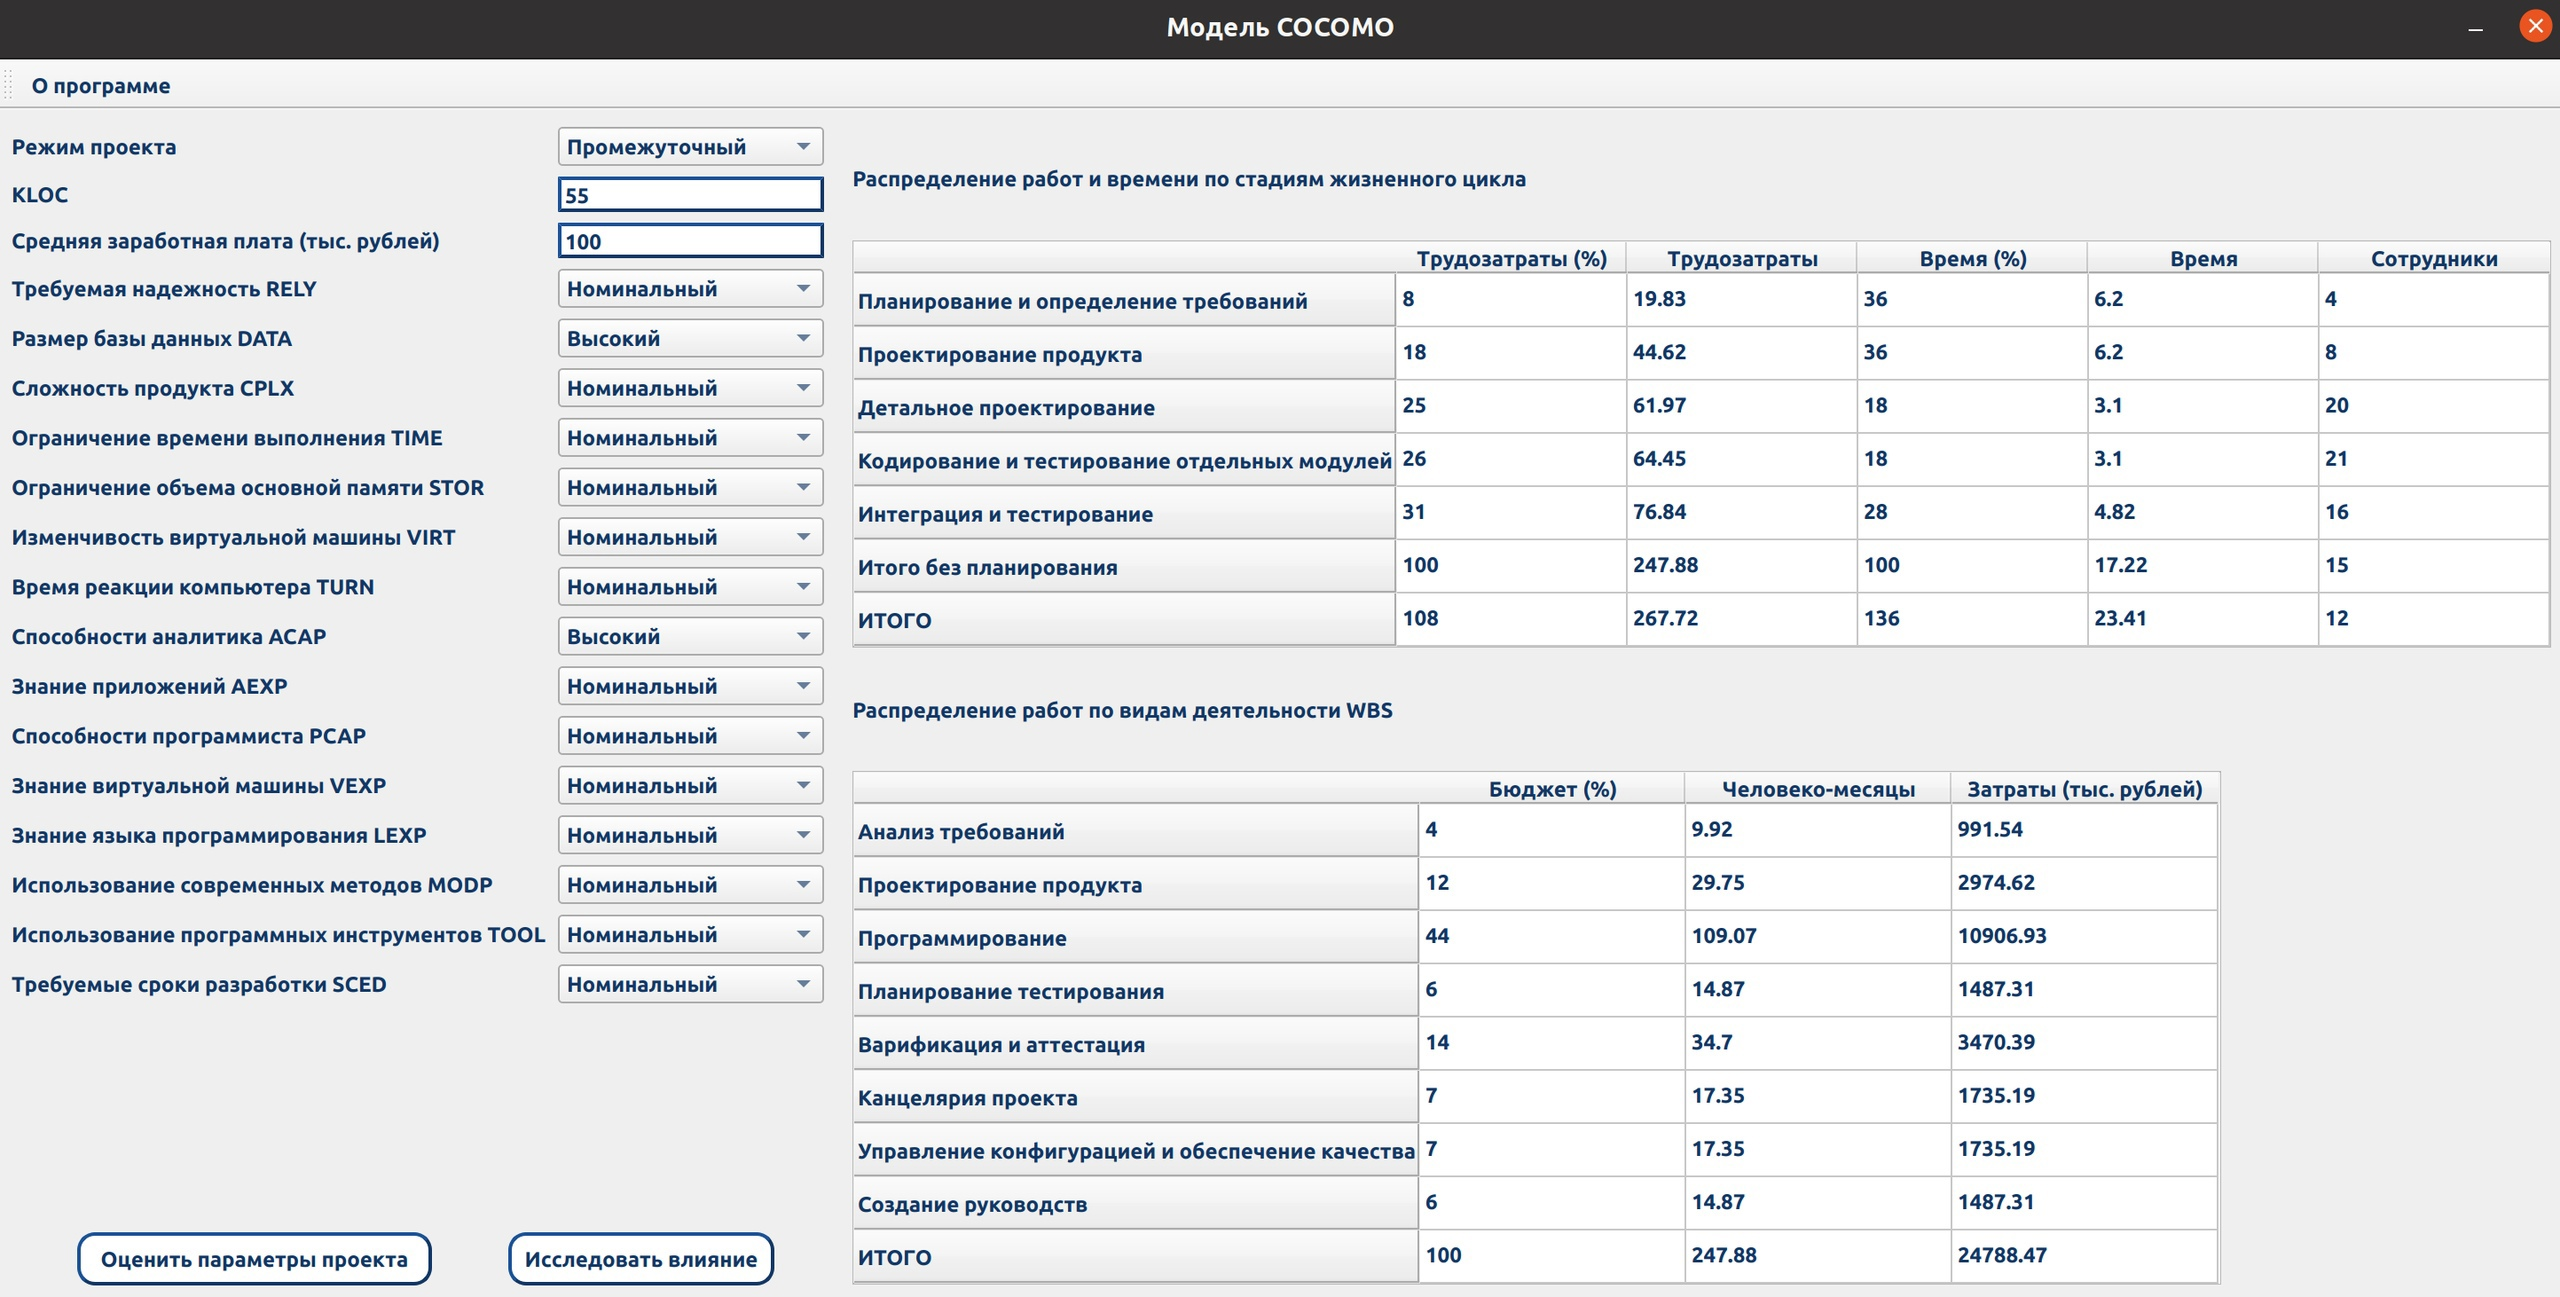
\includegraphics[scale=0.18]{inc/img/task2.jpg}
	\end{center}
	\captionsetup{justification=centering}
	\caption{Оценка параметров проекта с использованием COCOMO}
	\label{img:task2}
\end{figure}

Требуемое для этапа выполнения проекта число сотрудников вычисляется следующим образом:

\begin{equation}
	\text{Число} = \frac{\text{Трудозатраты}}{\text{Время}}.
\end{equation}

На рисунке \ref{img:task2-bar} показана диаграмма привлечения сотрудников, где

\begin{itemize}
	\item 1 --- планирование и определение требований;
	\item 2 --- проектирование продукта;
	\item 3 --- детальное проектирование;
	\item 4 --- кодирование и тестирование отдельных модулей;
	\item 5 --- интеграция и тестирование.
\end{itemize}

\begin{figure}[H]
	\begin{center}
		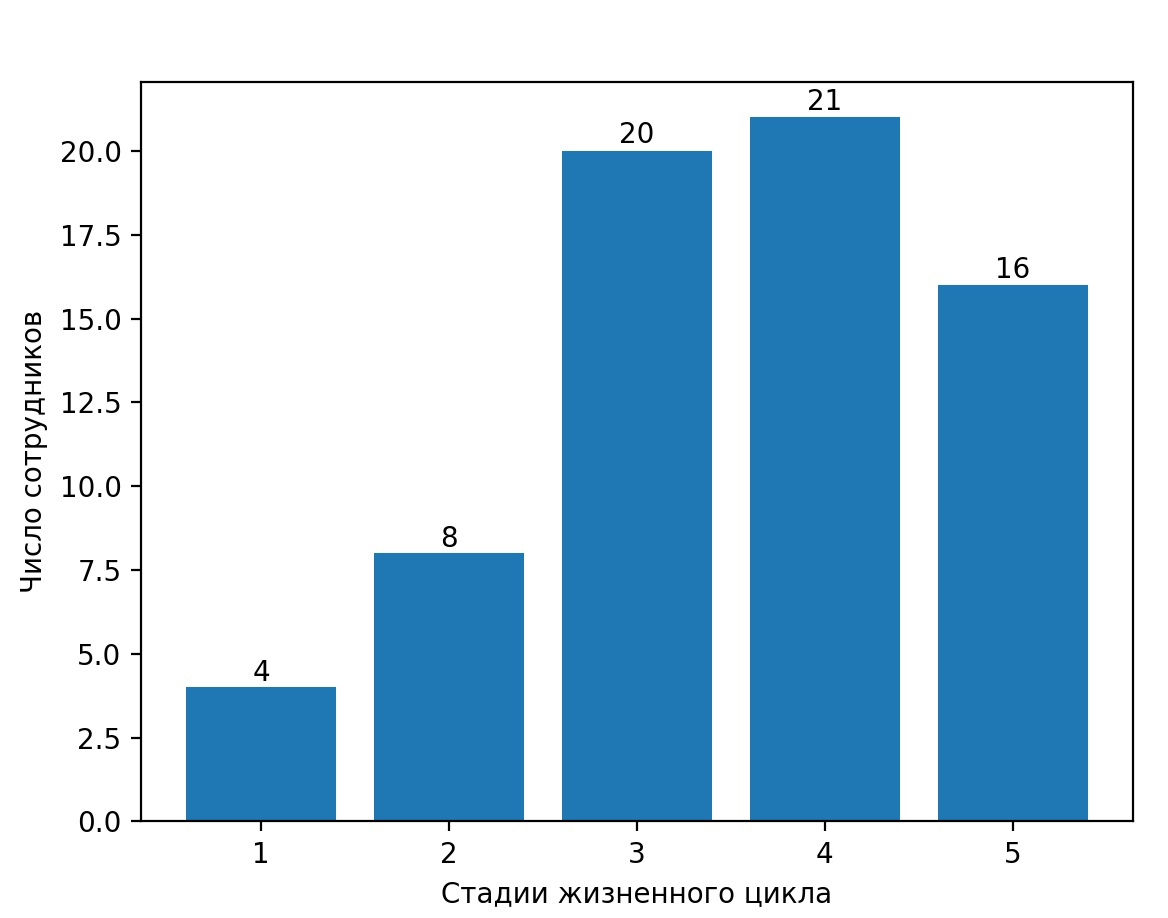
\includegraphics[scale=0.22]{inc/img/task2-bar.jpg}
	\end{center}
	\captionsetup{justification=centering}
	\caption{Диаграмма привлечения сотрудников}
	\label{img:task2-bar}
\end{figure}

Предварительную оценку бюджета проекта можно определить так:

\begin{equation}
	\text{Бюджет} = \text{Трудозатраты}\cdot\text{Средняя заработная плата}.
\end{equation}

Для средней заработной платы 100 000 рублей проект обойдется в 2 4788 470 рублей.

\subsubsection*{Выводы}

Анализ распределения работ и времени по стадиям жизненного цикла и распределения работ по видам деятельности WBS показал:

\begin{itemize}
	\item трудозатраты без учета планирования и определения требований составили 247.88 человеко-месяцев, с учетом --- 267.72 человеко-месяца;
	\item время без учета планирования и определения требований составило 17.22 месяцев, с учетом --- 23.41 месяца;
	\item для средней заработной платы 100 000 рублей проект обойдется в 2 4788 470 рублей;
	\item наибольшие затраты на <<Программирование>> --- 10 906 930 рублей, наименьшие затраты на <<Анализ требований>> --- 991 540 рублей;
	\item наибольшее число сотрудников необходимо для этапа <<Кодирование и тестирование отдельных модулей>> --- 21 человек, наименьшее число сотрудников необходимо для этапа <<Планирование и определение требования>> --- 4 человека.
\end{itemize}

\section*{Вывод}

При выполнении лабораторной работы были отработаны навыки предварительной оценки параметров программного проекта на примере методики COCOMO.

С использованием модели COCOMO можно выполнить предварительную оценку трудозатрат, длительности выполнения и стоимости проекта. При этом методика позволяет производить расчеты для проектов разных масштабов с учетом их индивидуальных характеристик и проста в применении. Но у модели есть недостатки, влияющие на точность оценок:

\begin{itemize}
	\item расчеты в модели зависят от размера проекта, поэтому точность оценки проекта зависит от точности оценки размера;
	\item не учитывается повторное использование компонентов, что влияет на размер проекта;
	\item методика основана на каскадной модели жизненного цикла, поэтому не учитывает тонкости других методологий.
\end{itemize}
